% 110-52(110쪽) — 숫자판. 가로 5칸 + 「$\cdots$」 칸, 세로 5줄 + 「$\vdots$」 줄.
% 왼쪽 위 2×2 칸(1·2·3·4)이 원문처럼 노랗게 칠해진 田 모양이다. 스캔 화질이 낮아 TikZ 로 다시 그림.
% 칸의 수는 원문 그대로만 적고, 구하는 합(답)은 그림에서 읽히지 않게 넣지 않는다.
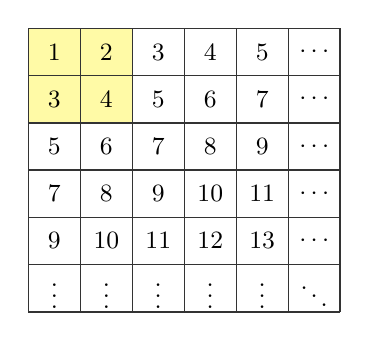
\begin{tikzpicture}[line width=0.5pt, x=1cm, y=1cm]
  \fill[yellow!35] (0,2.4) rectangle (1.32,3.6);
  \draw[black!80, xstep=0.66, ystep=0.6] (0,0) grid (3.96,3.6);
  \foreach \yc/\ca/\cb/\cc/\cd/\ce in {3.3/1/2/3/4/5, 2.7/3/4/5/6/7, 2.1/5/6/7/8/9, 1.5/7/8/9/10/11, 0.9/9/10/11/12/13}{
    \node[font=\small] at (0.33,\yc) {$\ca$};
    \node[font=\small] at (0.99,\yc) {$\cb$};
    \node[font=\small] at (1.65,\yc) {$\cc$};
    \node[font=\small] at (2.31,\yc) {$\cd$};
    \node[font=\small] at (2.97,\yc) {$\ce$};
    \node[font=\small] at (3.63,\yc) {$\cdots$};
  }
  \foreach \xc in {0.33, 0.99, 1.65, 2.31, 2.97}{
    \node[font=\small] at (\xc,0.3) {$\vdots$};
  }
  \node[font=\small] at (3.63,0.3) {$\ddots$};
\end{tikzpicture}
